\documentclass[11pt,aspectratio=169]{beamer}

% ========================================================================
% Packages
% ========================================================================
\usepackage[utf8]{inputenc}
\usepackage[T1]{fontenc}
\usepackage{amsmath,amssymb,amsthm}
\usepackage{graphicx}
\graphicspath{{../results/plots/}{../results/run_PPO_seed42/plots/}}
\usepackage{booktabs}
\usepackage{hyperref}
\usepackage{xcolor}
\usepackage{listings}
\usepackage{float}
\usepackage{multirow}
\usepackage{makecell}
\usepackage{tikz}
\usepackage{pgfplots}
\usepackage{pifont}
\pgfplotsset{compat=1.18}

% ========================================================================
% Beamer Theme & Colors
% ========================================================================
\usetheme{Madrid}
\usecolortheme{default}

\definecolor{IITBlue}{RGB}{0,51,102}
\definecolor{IITGold}{RGB}{204,153,0}
\definecolor{codegray}{RGB}{240,240,240}

\setbeamercolor{structure}{fg=IITBlue}
\setbeamercolor{title}{fg=IITBlue}
% The frame title sits on the IIT blue title bar, so its text has to be white.
% In IIT blue it was invisible on every frame.
\setbeamercolor{frametitle}{fg=white}
\setbeamercolor{block title}{bg=IITBlue,fg=white}
\setbeamercolor{block body}{bg=IITBlue!10,fg=black}
\setbeamercolor{alerted text}{fg=IITGold}

\setbeamertemplate{navigation symbols}{}
\setbeamertemplate{footline}[frame number]

% ========================================================================
% Custom commands
% ========================================================================
\newcommand{\vc}[1]{\boldsymbol{#1}}
\newcommand{\R}{\mathbb{R}}
\newcommand{\E}{\mathbb{E}}
\newcommand{\argmax}{\mathop{\mathrm{argmax}}}
\newcommand{\argmin}{\mathop{\mathrm{argmin}}}
\newcommand{\MRR}{\mathrm{MRR}}
\newcommand{\Ra}{R_a}
\newcommand{\RaSafe}{R_{a,\text{safe}}}
\newcommand{\RaMax}{R_{a,\text{max}}}
\newcommand{\RaFinal}{R_{a,\text{final}}}
\newcommand{\VB}{V_B}
\newcommand{\VBMax}{V_{B,\text{max}}}
\newcommand{\VBSafe}{V_{B,\text{safe}}}
\newcommand{\CMark}{\ding{51}}
\newcommand{\XMark}{\ding{55}}

\lstdefinestyle{bash}{
    backgroundcolor=\color{codegray},
    basicstyle=\ttfamily\scriptsize,
    breaklines=true,
    frame=single,
    framerule=0.5pt,
    rulecolor=\color{IITBlue!30}
}

% ========================================================================
% Title Page Info
% ========================================================================
\title[Digital Twin DRL for CNC Milling]{Digital Twin-Driven Deep Reinforcement Learning\\for Energy-Aware CNC Milling Parameter Optimization}
\subtitle{ME6324 -- AI in Manufacturing \textbar\ Course Project}
\author{Abhinand \\ Department of Mechanical Engineering \\ Indian Institute of Technology Madras}
\institute{IIT Madras}
\date{\today \\ Git Revision: \texttt{d76603b}}

% ========================================================================
% Document
% ========================================================================
\begin{document}

% ---------- Title Slide ----------
\begin{frame}
    \titlepage
    \vfill
    \centering
    \small \textit{All results reproducible from committed artifacts}
\end{frame}

% ---------- Table of Contents ----------
\begin{frame}{Outline}
    \tableofcontents
\end{frame}

% ========================================================================
% SECTION 1: INTRODUCTION
% ========================================================================
\section{Introduction}

\begin{frame}{Problem: Dynamic Cutting Parameter Optimization}
    CNC face milling: rotating cutter removes material in multiple passes.
    \vspace{0.5em}

    \textbf{Parameters to optimize:}
    \begin{itemize}
        \item Spindle speed $n$ [RPM]
        \item Feed per revolution $f_r$ [mm/r]
        \item Axial depth of cut $a_p$ [mm]
    \end{itemize}

    \vspace{0.5em}
    \textbf{Four competing objectives:}
    \begin{itemize}
        \item \textbf{Productivity:} Maximize $\MRR = v_c \cdot a_p \cdot f_r$
        \item \textbf{Energy:} Minimize total electrical energy/part
        \item \textbf{Quality:} $\Ra \le 1.6\ \mu\text{m}$ (finished surface)
        \item \textbf{Tool Life:} $\VB \le 0.3\ \text{mm}$, avoid breakage
    \end{itemize}

    \vspace{0.5em}
    \alert{Traditional fixed parameters (handbooks, static NSGA-II) cannot adapt to tool wear, material variation, or geometry changes.}
\end{frame}

\begin{frame}{Proposed Approach}
    \small
    \begin{columns}[T]
        \begin{column}{0.5\textwidth}
            \textbf{1. Digital Twin (Physics)}
            \begin{itemize}
                \item Speed-dependent cutting energy $k_c(v_c) = k_{c0}(v_c/v_{\text{ref}})^m$
                \item Extended Taylor tool wear
                \item Empirical roughness regression
                \item Stochastic breakage
            \end{itemize}

            \textbf{2. DRL Agent (PPO)}
            \begin{itemize}
                \item One Gymnasium environment
                \item 11-D observation, context always present
                \item Energy-aware reward
                \item Conditioned policy ($w_2$ + material context)
            \end{itemize}
        \end{column}
        \begin{column}{0.5\textwidth}
            \textbf{3. Experimental Rigor}
            \begin{itemize}
                \item 100-scenario Monte Carlo + 95\% CIs
                \item Ablation: 7 weights $\times$ 3 seeds
                \item 5 classical baselines + receding-horizon
                \item Transfer experiment
                \item Full reproducibility
            \end{itemize}

            \textbf{4. Interactive Workstation}
            \begin{itemize}
                \item 2D stock depletion, micro-topography
                \item G-code generation, multi-controller comparison
            \end{itemize}
        \end{column}
    \end{columns}
\end{frame}

% ========================================================================
% SECTION 2: RELATED WORK
% ========================================================================
\section{Related Work}

\begin{frame}{Positioning Against Reference Papers}
    \begin{table}
    \centering
    \label{tab:papers}
    \scriptsize
    \begin{tabular}{@{}lccc@{}}
    \toprule
\textbf{Capability} & \makecell{Mo et al. (2025)\\\textsl{J. Manuf. Process 156}} & \makecell{Wang et al. (2025a)\\\textsl{J. Manuf. Syst. 78}} & \textbf{This Work} \\
    \midrule
    Dynamic optimization & \CMark & \CMark & \CMark \\
    Tool wear in the state & \CMark & \XMark & \CMark \\
    Roughness constraint & \CMark & \XMark & \CMark \\
    Energy as an objective & \XMark & \XMark & \CMark \\
    Speed-dependent $k_c$ & \XMark & \XMark & \CMark \\
    Domain randomization & \XMark & \XMark & \CMark \\
    Conditioned policy & \XMark & \XMark & \CMark \\
    Transfer experiment & \XMark & \XMark & \CMark \\
    Receding-horizon baseline & \XMark & \XMark & \CMark \\
    Monte Carlo (100 scenarios) & \XMark & \XMark & \CMark \\
    Interactive workstation & \XMark & \XMark & \CMark \\
    \bottomrule
    \end{tabular}
    \end{table}

    \vspace{0.4em}
    \scriptsize
    Mo \emph{et al.}: PPO over a mixed action space (tool change + parameters); the state carries
    $\VB$, breakage and $\Ra$; objectives are quality and efficiency.\\
    Wang \emph{et al.}: MATD3 for batch milling; objectives are dimensional quality and machining time.

    \vspace{0.3em}
    \alert{Key differentiator:} \textbf{neither reference treats energy as an objective}. The
    speed-dependent $k_c$ creates a genuine energy/throughput trade-off, and one conditioned
    policy covers the whole frontier in a single run.
\end{frame}

% ========================================================================
% SECTION 3: PHYSICS
% ========================================================================
\section{Digital Twin Physics}

\begin{frame}{Key Physics Equations (MillingDT/config/physics.py)}
    \begin{columns}[T]
        \begin{column}{0.55\textwidth}
            \begin{align}
                v_c &= \frac{\pi D n}{1000} \\
                \MRR &= v_c \cdot a_p \cdot f_r \\
                t_{\text{cut}} &= \frac{L_{\text{cut}}}{n f_r} \\
                \Delta \VB &= C_{\text{wear}} v_c^{\alpha} f_r^{\beta} a_p^{\gamma} t_{\text{cut}} \\
                \Ra &= k_1 f_r^2 + k_2 \VB + \frac{k_3}{v_c} \\
                k_c(v_c) &= k_{c0} \left( \frac{v_c}{v_{\text{ref}}} \right)^m \\
                P_{\text{total}} &= P_{\text{idle}} + k_c(v_c) \cdot \MRR \\
                E_{\text{pass}} &= P_{\text{total}} \cdot t_{\text{cut}}
            \end{align}
        \end{column}
        \begin{column}{0.45\textwidth}
            \begin{alertblock}{Key Insight: Interior Minimum}
            With $m=0.6 > 0$:
            \begin{itemize}
                \item Idle energy $\propto 1/(n f_r)$ $\downarrow$ with speed
                \item Cutting energy $\propto n^m$ $\uparrow$ with speed
                \item Part energy $E_{\text{part}}(v_c)$ has \textbf{interior minimum}
                \item Energy weight $w_2$ selects operating point
            \end{itemize}
            Validated by a unit test on the part energy minimum
            \end{alertblock}
        \end{column}
    \end{columns}
\end{frame}

% ========================================================================
% SECTION 4: ENVIRONMENT
% ========================================================================
\section{Environment Design}

\begin{frame}{One Gymnasium Environment: \texttt{MillingDTEnv-v1}}
    \footnotesize
    \begin{columns}[T]
        \begin{column}{0.5\textwidth}
            \textbf{One registration}
            \begin{itemize}
                \item \texttt{env.ENV\_ID} = \texttt{MillingDTEnv-v1}, 200-step limit
                \item The energy weight and the material are \emph{inputs}, not separate tasks
            \end{itemize}

            \textbf{Observation (11-D, always the same shape)}
            \begin{itemize}
                \item 0--7: $\tanh$-squashed $\VB$, $\kappa_{\text{rem}}$, previous $n, f_r, a_p$,
                      $\MRR/\MRR_{\text{max}}$, $\tanh$-squashed $\Ra$, tool-broken flag
                \item 8--10: the context: $w_2$, $C_\text{wear}$ over $[0.6,1.4]$,
                      $k_1$ over $[0.8,1.2]$ of nominal
            \end{itemize}

            \textbf{Action:} $[-1,1]^3$ $\to$ clipped $\to$ machine envelope
        \end{column}
        \begin{column}{0.5\textwidth}
            \textbf{Reward per step}
            \setlength{\jot}{3pt}
            \begin{align}
                r = &\ 5\left(w_1 \frac{\MRR}{\MRR_\text{max}} - w_2 \frac{E_\text{pass}}{E_\text{ref}}\right)
                    + 2\,\Delta\!\left(\tfrac{\kappa_\text{removed}}{\kappa_\text{total}}\right) \\
                    &- 50\,\mathbb{1}[\VB > \VBSafe] - 100\,\mathbb{1}[\text{broken}] \\
                    &- 50\,\mathbb{1}[\text{finish} \wedge \Ra > \RaSafe] - 0.05
            \end{align}
            \vspace{0.2em}
            \begin{itemize}
                \item $+200$ when a part is finished in spec, plus a Pareto margin bonus of at most $+5$
                \item $w_1 = 1 - w_2$; safety limits $\VBSafe = 0.255$ mm and $\RaSafe = 1.36\ \mu$m
                \item breakage $p = 0.3 \cdot$ wear factor $\cdot$ (load factor)$^2$ above $\VB > 0.15$ mm
                \item the objective scale of $5$ lets $w_2$ compete with the shaping terms
            \end{itemize}
        \end{column}
    \end{columns}
\end{frame}

\begin{frame}{Domain Randomization}
    \begin{itemize}
        \item \textbf{Workpiece:} $\kappa_{\text{total}} \in [2,15]$, $D \in [40,150]$, $L_{\text{cut}} \in [50,200]$
        \item \textbf{Material/Tool:} $C_\text{wear}$ at $[0.6,1.4]\times$ nominal, $k_1, k_2, k_3$ at $[0.8,1.2]\times$ nominal
        \item \textbf{Initial wear:} $V_{B,0} \sim \mathcal{U}[0, 0.8] V_{B,\text{max}}$
        \item \textbf{Energy weight:} drawn $\mathcal{U}[0,1]$ per episode under \texttt{--randomize-weight}
        \item \textbf{Shared tables:} same \texttt{MillingDT/config/scenarios.py} for training + Monte Carlo eval
        \item \smallskip
        \item \textbf{Measured:} the normalized physics features the policy sees on the training and the evaluation sets agree to 0.041 in the mean (std = 1), the same distribution
        \item \textbf{In the observation:} $C_\text{wear}$ and $k_1$ travel with the part, so the policy knows which material it is cutting
    \end{itemize}
\end{frame}

% ========================================================================
% SECTION 5: RL
% ========================================================================
\section{Reinforcement Learning}

\begin{frame}{PPO Training Setup (Stable-Baselines3)}
    \begin{columns}[T]
        \begin{column}{0.5\textwidth}
            \begin{table}
            \centering
            \scriptsize
            \caption{Hyperparameters}
            \begin{tabular}{@{}ll@{}}
            \toprule
            \textbf{Parameter} & \textbf{Value} \\
            \midrule
            Policy & MlpPolicy (2$\times$256) \\
            Learning rate & $3\times10^{-4}$ (linear) \\
            $n\_steps$ & 2048 \\
            Batch size & 64 \\
            $n\_epochs$ & 10 \\
            $\gamma$ / GAE $\lambda$ & 0.99 / 0.95 \\
            Clip range & 0.2 \\
            Entropy coeff & 0.02 \\
            VecNormalize & norm\_obs=True, norm\_reward=True \\
            Envs / Device & 4 (\texttt{SubprocVecEnv}) / CPU \\
            \bottomrule
            \end{tabular}
            \end{table}
        \end{column}
        \begin{column}{0.5\textwidth}
            \textbf{Training Runs}
            \begin{itemize}
                \item \textbf{Production policy:} 1M steps, seed 42,
                      \texttt{--randomize --randomize-weight}
                      $\to$ \texttt{results/run\_PPO\_seed42/}
                \item \textbf{Ablation grid:} 7 $w_2$ $\times$ 3 seeds = 21 policies,
                      150k steps each
            \end{itemize}

            \vspace{0.3em}
            \footnotesize
            Every ablation policy has its energy weight \alert{pinned} at training and is
            \alert{evaluated at that same weight}, so a policy is always asked the question it
            was trained for. The production policy instead sees the weight drawn per episode.

            \vspace{0.6em}
            \alert{Heartbeat callback} every 1000 steps $\to$ stall detection in \texttt{run\_experiments.py}
        \end{column}
    \end{columns}
\end{frame}

% ========================================================================
% SECTION 6: RESULTS
% ========================================================================
\section{Results}

\begin{frame}{Production Policy: Monte Carlo Sweep (100 Scenarios)}
    \small
    \begin{columns}[T]
        \begin{column}{0.5\textwidth}
            \centering
            \scriptsize
            \begin{tabular}{@{}lrrr@{}}
            \toprule
            \textbf{Metric} & \textbf{Mean} & \textbf{Std} & \textbf{95\% CI} \\
            \midrule
            $\MRR$ (mm$^3$/min) & 1205.2 & 585.7 & [1088.9, 1321.4] \\
            Energy (kJ) & 68.4 & 48.3 & [58.8, 77.9] \\
            Cycle time (s) & 20.3 & 17.1 & [16.9, 23.6] \\
            Max $\Ra$ ($\mu$m) & 1.379 & 0.350 & [1.309, 1.448] \\
            Max $\VB$ (mm) & 0.1244 & 0.0679 & [0.1109, 0.1378] \\
            \bottomrule
            \end{tabular}
        \end{column}
        \begin{column}{0.5\textwidth}
            \centering
            \scriptsize
            \begin{tabular}{@{}lrr@{}}
            \toprule
            \textbf{Constraint} & \textbf{Rate} & \textbf{95\% CI} \\
            \midrule
            $\Ra$ viol., worst pass & 38.0\% & [28.5, 47.5]\% \\
            $\Ra$ viol., finished surface & \alert{0.0\%} & [0, 0]\% \\
            $\Ra$ above safety limit, worst & 56.0\% & [46.3, 65.7]\% \\
            $\Ra$ above safety limit, finished & \alert{0.0\%} & [0, 0]\% \\
            $\VB > 0.3$ mm & \alert{0.0\%} & [0, 0]\% \\
            Tool breakage & 1.0\% & [0, 3]\% \\
            Parts completed in spec & 99.0\% & \\
            \bottomrule
            \end{tabular}
        \end{column}
    \end{columns}

    \vspace{0.6em}
    \begin{block}{Key Findings}
    \footnotesize
    \begin{itemize}
        \item \alert{Finished surface always in spec} (0\% violations), the part quality holds
        \item \alert{Wear never exceeded} (0\% violations), 99\% of the parts completed
        \item 56\% of the passes exceed the safety margin $\RaSafe = 1.36\ \mu$m: the policy pushes and recovers by the finish pass
        \item Mean operating point: 7199 RPM, 0.247 mm/r, 2.11 mm, 4.0 passes
    \end{itemize}
    \end{block}
\end{frame}

\begin{frame}{Energy Weight Ablation: Empirical Pareto Frontier}
    \small
    \begin{table}
    \centering
    \scriptsize
    \caption{Ablation: mean $\pm$ std over 3 seeds, 50 scenarios each, weight pinned}
    \begin{tabular}{@{}ccccccc@{}}
    \toprule
    $w_2$ & $\MRR$ & Energy (kJ) & Cycle (s) & $n$ (RPM) & $f_r$ & Frontier \\
    \midrule
    0.0 & 946.3$\pm$63.4 & 82.9$\pm$1.4 & 44.8 & 7094 & 0.166 & dominated \\
    0.2 & 1007.8$\pm$22.7 & 77.1$\pm$1.1 & 31.3 & 7471 & 0.184 & dominated \\
    0.4 & 1038.0$\pm$67.6 & 72.7$\pm$0.5 & 24.8 & 7256 & 0.203 & \CMark \\
    0.5 & 1035.8$\pm$43.8 & 70.3$\pm$1.2 & 22.0 & 7080 & 0.214 & \CMark \\
    0.6 & 1023.9$\pm$27.4 & 70.8$\pm$0.6 & 22.1 & 7148 & 0.209 & dominated \\
    0.8 & 971.1$\pm$43.2 & 66.8$\pm$1.2 & 21.9 & 6538 & 0.228 & \CMark \\
    1.0 & 951.3$\pm$54.7 & 65.8$\pm$0.6 & 20.9 & 6490 & 0.229 & \CMark \\
    \bottomrule
    \end{tabular}
    \end{table}

    \vspace{0.4em}
    \begin{alertblock}{Frontier Analysis}
    From $w_2 = 0.4$ to $w_2 = 1.0$: the removal rate falls \alert{8.4\%} (1038 $\to$ 951 mm$^3$/min)
    and the energy falls \alert{9.5\%} (72.7 $\to$ 65.8 kJ). The trade-off is \textbf{symmetric}.
    The spindle speed falls with the energy weight (7256 $\to$ 6490 RPM): the energy is bought with
    throughput, not with time. Dominated points ($w_2 = 0.0, 0.2, 0.6$) remove less for more.
    \end{alertblock}
\end{frame}

\begin{frame}{Ablation Frontier: Removal Rate against Energy}
    \centering
    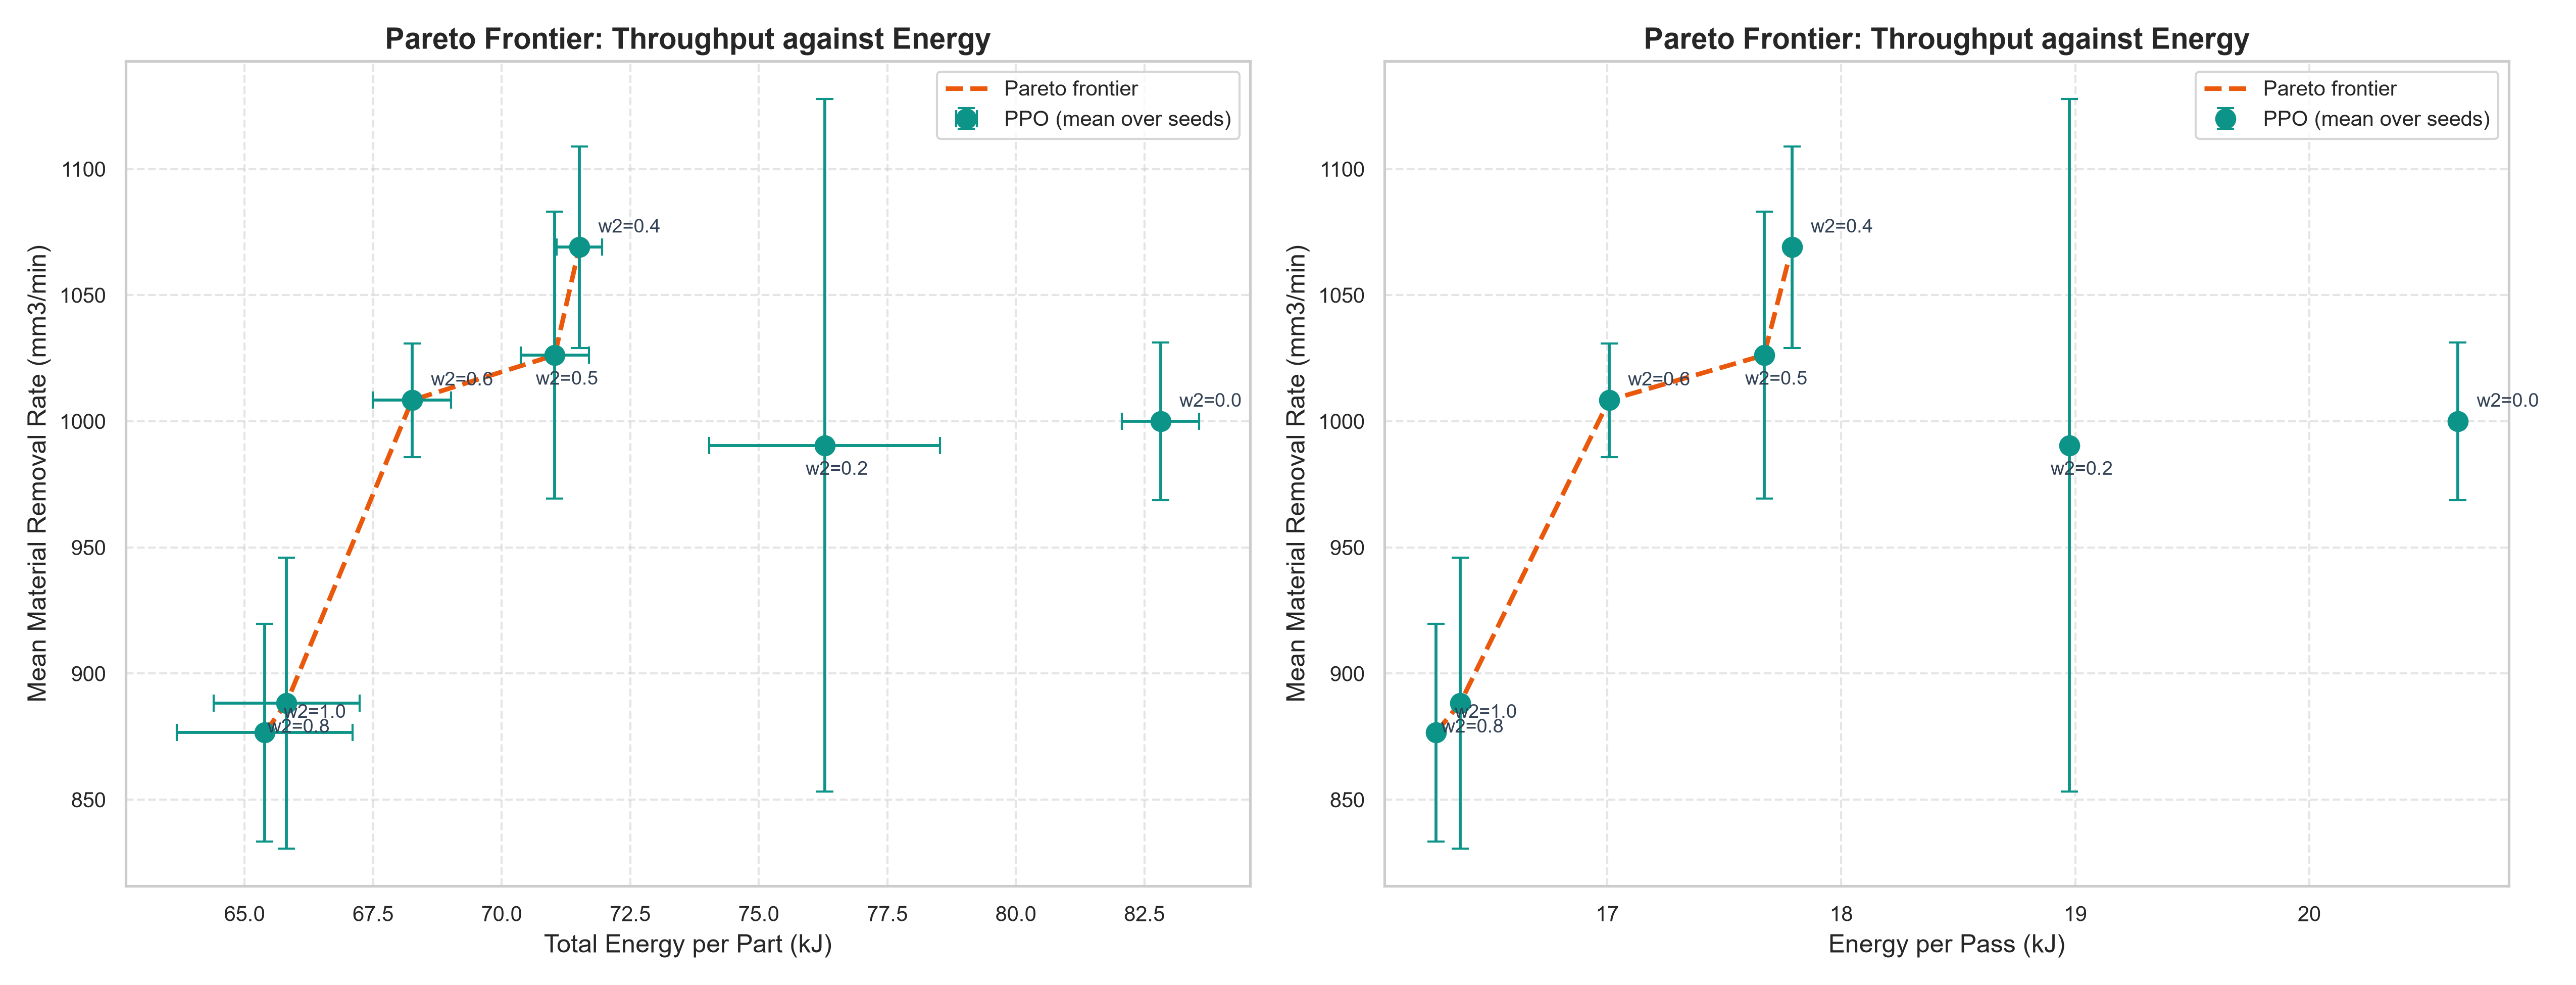
\includegraphics[width=\textwidth,height=0.66\textheight,keepaspectratio]{ablation_pareto_frontier.png}

    \vspace{0.3em}
    {\footnotesize
    Seven pinned-weight policies, three seeds each. \alert{The four non-dominated points are joined into
    the frontier}: $w_2 = 0.4$, $0.5$, $0.8$, $1.0$, and the three dominated points sit off it.
    Left panel: the energy of a part. Right panel: the energy of a pass, which the reward charges.}
\end{frame}

\begin{frame}{One Policy Against 21 Policies}
    \small
    \begin{table}
    \centering
    \scriptsize
    \begin{tabular}{@{}rrrrrrr@{}}
    \toprule
    $w_2$ & \makecell{$\MRR$, one\\policy} & \makecell{$\MRR$, per\\weight} & $\MRR$ gap
           & \makecell{Energy, one\\policy} & \makecell{Energy, per\\weight} & Energy gap \\
    \midrule
    0.0 & 1213.6 & 946.3 & $+28.2\%$ & 69.6 & 82.9 & $-16.0\%$ \\
    0.2 & 1215.3 & 1007.8 & $+20.6\%$ & 69.0 & 77.1 & $-10.5\%$ \\
    0.4 & 1205.1 & 1038.0 & $+16.1\%$ & 68.3 & 72.7 & $-6.0\%$ \\
    0.5 & 1191.0 & 1035.8 & $+15.0\%$ & 68.0 & 70.3 & $-3.3\%$ \\
    0.6 & 1169.3 & 1023.9 & $+14.2\%$ & 67.6 & 70.8 & $-4.5\%$ \\
    0.8 & 1130.8 & 971.1 & $+16.4\%$ & 67.1 & 66.8 & $+0.5\%$ \\
    1.0 & 1096.0 & 951.3 & $+15.2\%$ & 67.1 & 65.8 & $+2.1\%$ \\
    \bottomrule
    \end{tabular}
    \end{table}

    \vspace{0.3em}
    \begin{block}{Result}
    \small
    For $w_2$ from 0.0 to 0.6 the single policy removes \alert{14\% to 28\%} more material for
    \alert{3\% to 16\%} less energy. At $w_2 = 0.8$ and $w_2 = 1.0$ it still removes 16\% and 15\%
    more for 0.5\% and 2.1\% more energy.
    \end{block}

    \vspace{0.1em}
    \footnotesize
    The same policy swept at runtime: $\MRR$ 1213.6 ($w_2=0.0$) $\to$ 1096.0 ($w_2=1.0$), energy
    69.6 $\to$ 67.1 kJ, spindle 7513 $\to$ 6475 RPM. \textbf{The weight stays a runtime query}, not a
    retrain: the observation carries $w_2$ and the material context ($C_\text{wear}$, $k_1$).
\end{frame}

\begin{frame}{Baseline Comparison (50 Episodes, Nominal Condition, $w_2 = 0.4$)}
    \begin{table}
    \centering
    \scriptsize
    \caption{Baseline comparison on the same 50 episodes}
    \begin{tabular}{@{}lcccc@{}}
    \toprule
    \textbf{Policy} & \textbf{Reward} & \textbf{$\MRR$} & \textbf{Energy (kJ)} & \textbf{Cycle (s)} \\
    \midrule
    PPO (ours) & 204.09 & 894.3 & 18.40 & 5.56 \\
    \textbf{Receding-Horizon} & 203.45 & \textbf{981.7} & \textbf{18.02} & \textbf{4.80} \\
    NSGA-II Static & -46.39 & 732.9 & 18.8 & 6.4 \\
    Rule-Based & -46.48 & 719.8 & 18.7 & 6.6 \\
    Constant-High & -46.10 & 1099.6 & 17.8 & 4.3 \alert{(violates)} \\
    Constant-Safe & -139.25 & 1.6 & 1506.8 & 3000.0 \\
    \bottomrule
    \end{tabular}
    \end{table}

    \vspace{0.5em}
    \begin{itemize}
        \item \textbf{Same 50 episodes} of the nominal condition for all six policies, at $w_2 = 0.4$
        \item \textbf{Level on the reward:} PPO 204.1 against the controller 203.5
        \item \textbf{The controller is ahead} on the removal rate (981.7 against 894.3) and the cycle time (4.80 s against 5.56 s)
        \item \alert{No reinforcement learning advantage is demonstrated yet}
        \item The three fast static policies finish outside the roughness safety limit, so the reward takes the $-50$ finishing penalty; Constant-Safe stays inside but needs 3000 s
    \end{itemize}
\end{frame}

\begin{frame}{Policy Comparison: Six Policies, Same 50 Episodes}
    \centering
    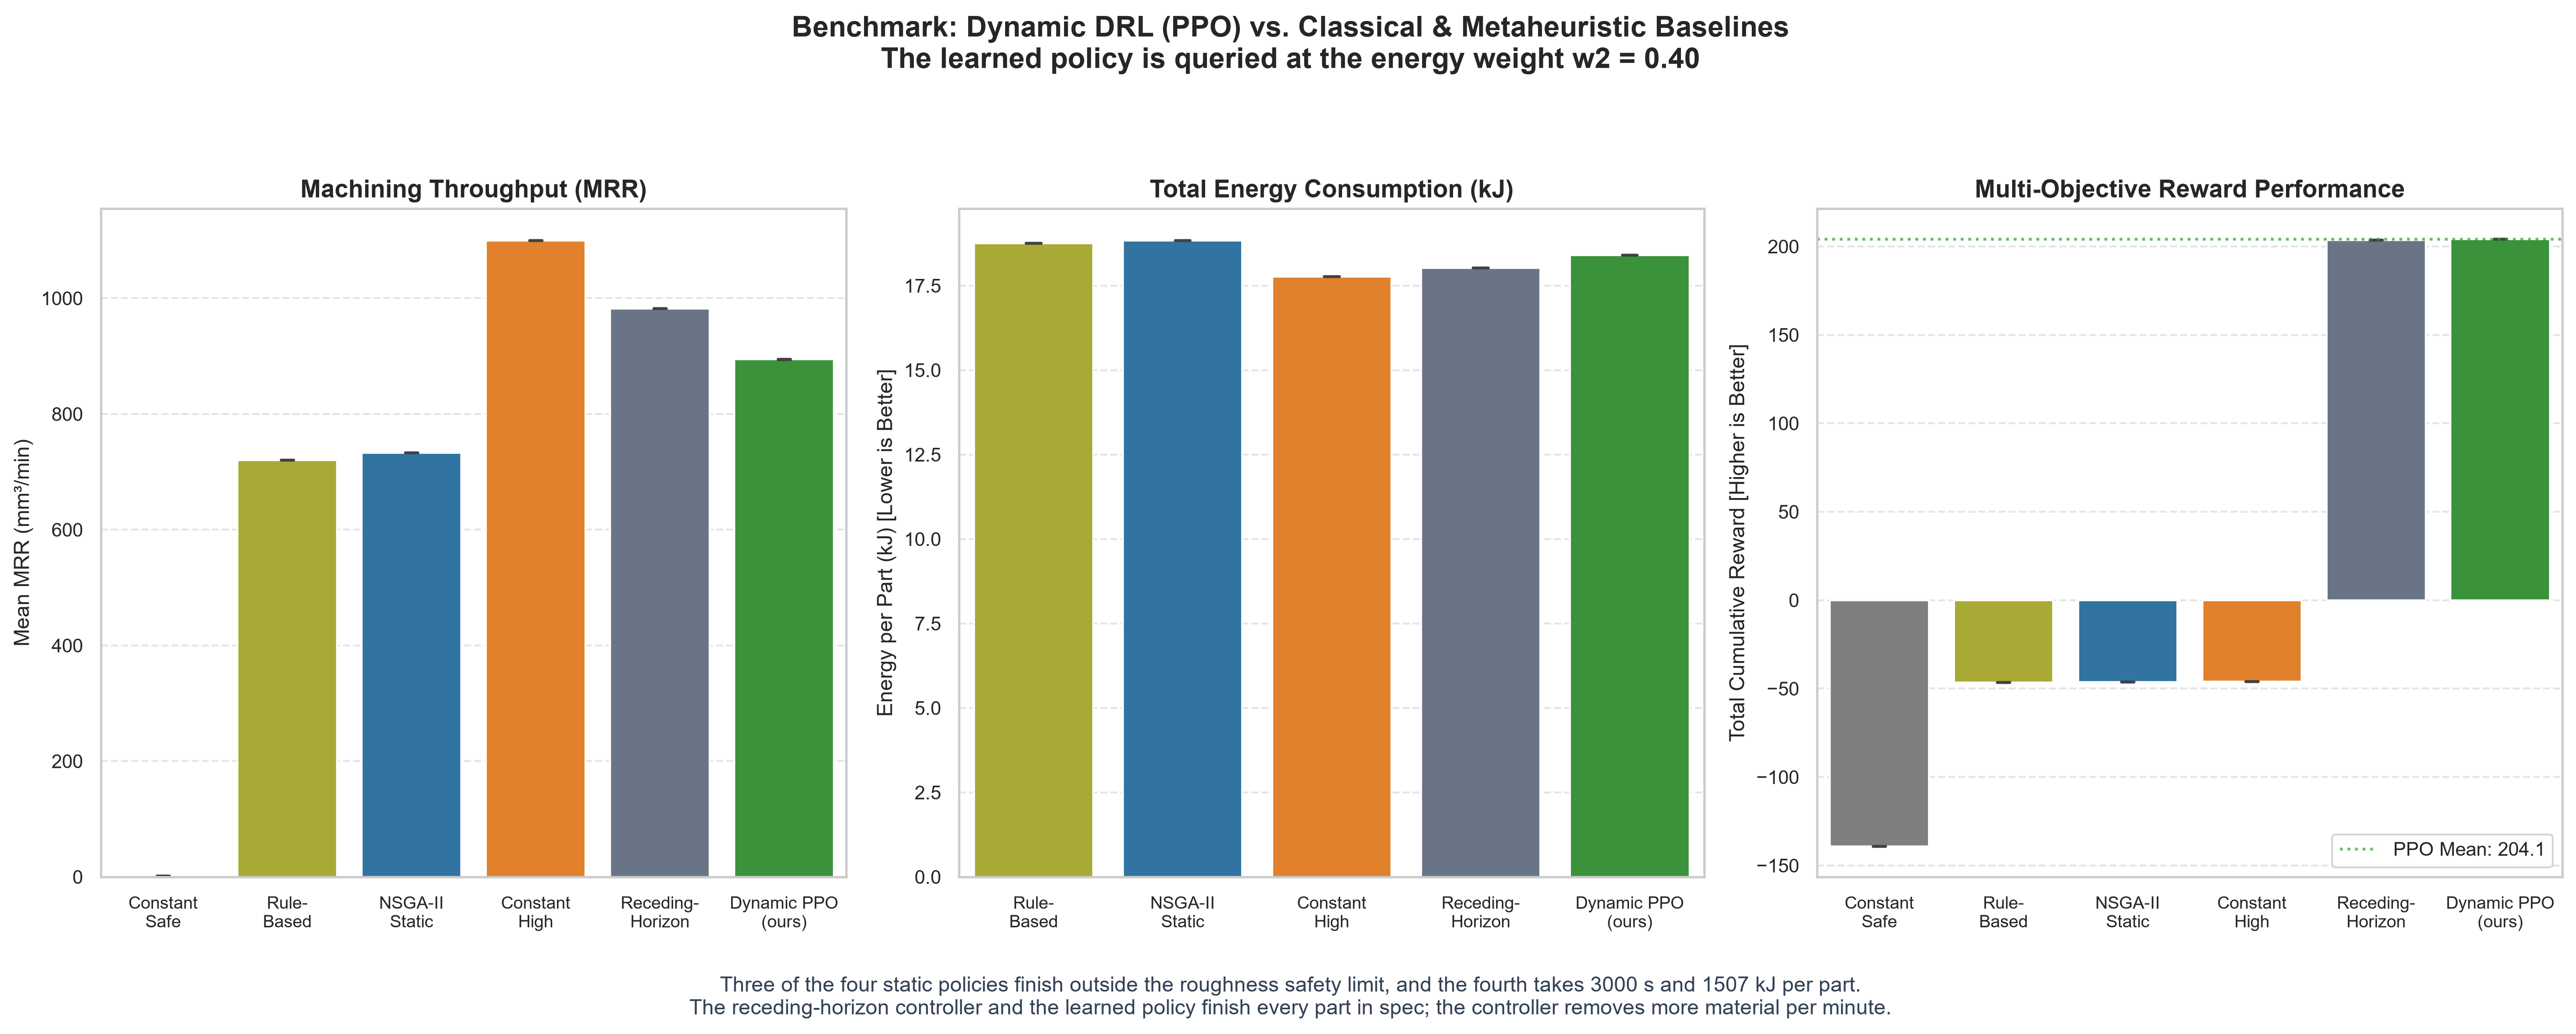
\includegraphics[width=\textwidth,height=0.66\textheight,keepaspectratio]{baseline_vs_ppo_comparison.png}

    \vspace{0.3em}
    {\footnotesize
    \alert{The four static policies all take a negative reward}: three of them finish outside the roughness
    safety limit and Constant-Safe stays inside but needs 3000 s per part. The comparison that matters is the
    receding-horizon controller against the learned policy, the only two with a positive reward.}
\end{frame}

\begin{frame}{Controller Initialization: Method and Result}
    \small
    \footnotesize\textbf{Question:} does a policy that starts from the controller end up better than the expert it started from?

    \begin{block}{Method}
    \footnotesize
    \begin{enumerate}
        \item Record the controller on 2000 randomized episodes
        \item Fit a supervised actor (2$\times$256, Tanh) on those trajectories by regression
        \item Copy the fitted weights into a fresh PPO policy
        \item Train with the production budget (1M steps), evaluate on 100 scenarios at $w_2 = 0.4$
    \end{enumerate}
    \footnotesize
    \texttt{MillingDT/agent/controller\_init.py} \quad \texttt{experiments/controller\_experiment.py}
    \end{block}

    \centering
    \scriptsize
    \begin{tabular}{@{}lccc@{}}
    \toprule
    \textbf{Metric} & \makecell{\textbf{Receding-horizon}\\\textbf{controller}} & \makecell{\textbf{PPO}\\\textbf{from scratch}} & \makecell{\textbf{PPO initialized}\\\textbf{from controller}} \\
    \midrule
    Mean episode reward & 187.96 & 198.57 & \alert{199.35} \\
    Reward std & 65.92 & 30.03 & \alert{3.35} \\
    $\MRR$ (mm$^3$/min) & \alert{1560.6} & 1205.1 & 1126.1 \\
    Energy per part (kJ) & 68.01 & 68.35 & 77.17 \\
    Cycle time (s) & \alert{13.54} & 20.25 & 32.35 \\
    Tool breakage & 5\% & 1\% & \alert{0\%} \\
    Parts completed & 95\% & 99\% & \alert{100\%} \\
    \bottomrule
    \end{tabular}
\end{frame}

\begin{frame}{Controller Initialization: What It Shows}
    \small
    \begin{columns}[T]
        \begin{column}{0.48\textwidth}
            \begin{alertblock}{No advantage over the controller}
            \footnotesize
            \begin{itemize}
                \item The controller still removes 38\% more material per minute (1560.6 against 1126.1 mm$^3$/min)
                \item and finishes in 13.5 s against 32.3 s
                \item The reward cannot separate the two learned policies: 199.35 against 198.57 is a gap of 0.8, while the standard error of the mean over 100 scenarios is $30.0/\sqrt{100} = 3.0$
                \item All three arms keep the finished surface in spec (0\% violations)
            \end{itemize}
            \end{alertblock}
        \end{column}
        \begin{column}{0.48\textwidth}
            \begin{block}{Consistency, paid for with throughput and energy}
            \footnotesize
            \begin{itemize}
                \item Reward std across the 100 scenarios falls from 30.0 to \alert{3.4}, tool breakage falls to \alert{zero}, every part is completed
                \item Against the from-scratch policy: 6.6\% less removal rate and 12.9\% more energy per part
                \item The controller is the least reliable arm of the three: std 65.9, 5\% breakage, 95\% of the parts completed
            \end{itemize}
            \end{block}
        \end{column}
    \end{columns}

    \vspace{0.4em}
    \begin{alertblock}{What the work claims}
    \footnotesize
    The reinforcement learning agent navigates the energy/throughput trade-off inside a fixed constraint set.
    It does not beat a classical controller that re-optimizes every pass with the exact physics.
    \end{alertblock}
\end{frame}

\begin{frame}{Controller Initialization: The Three Arms}
    \centering
    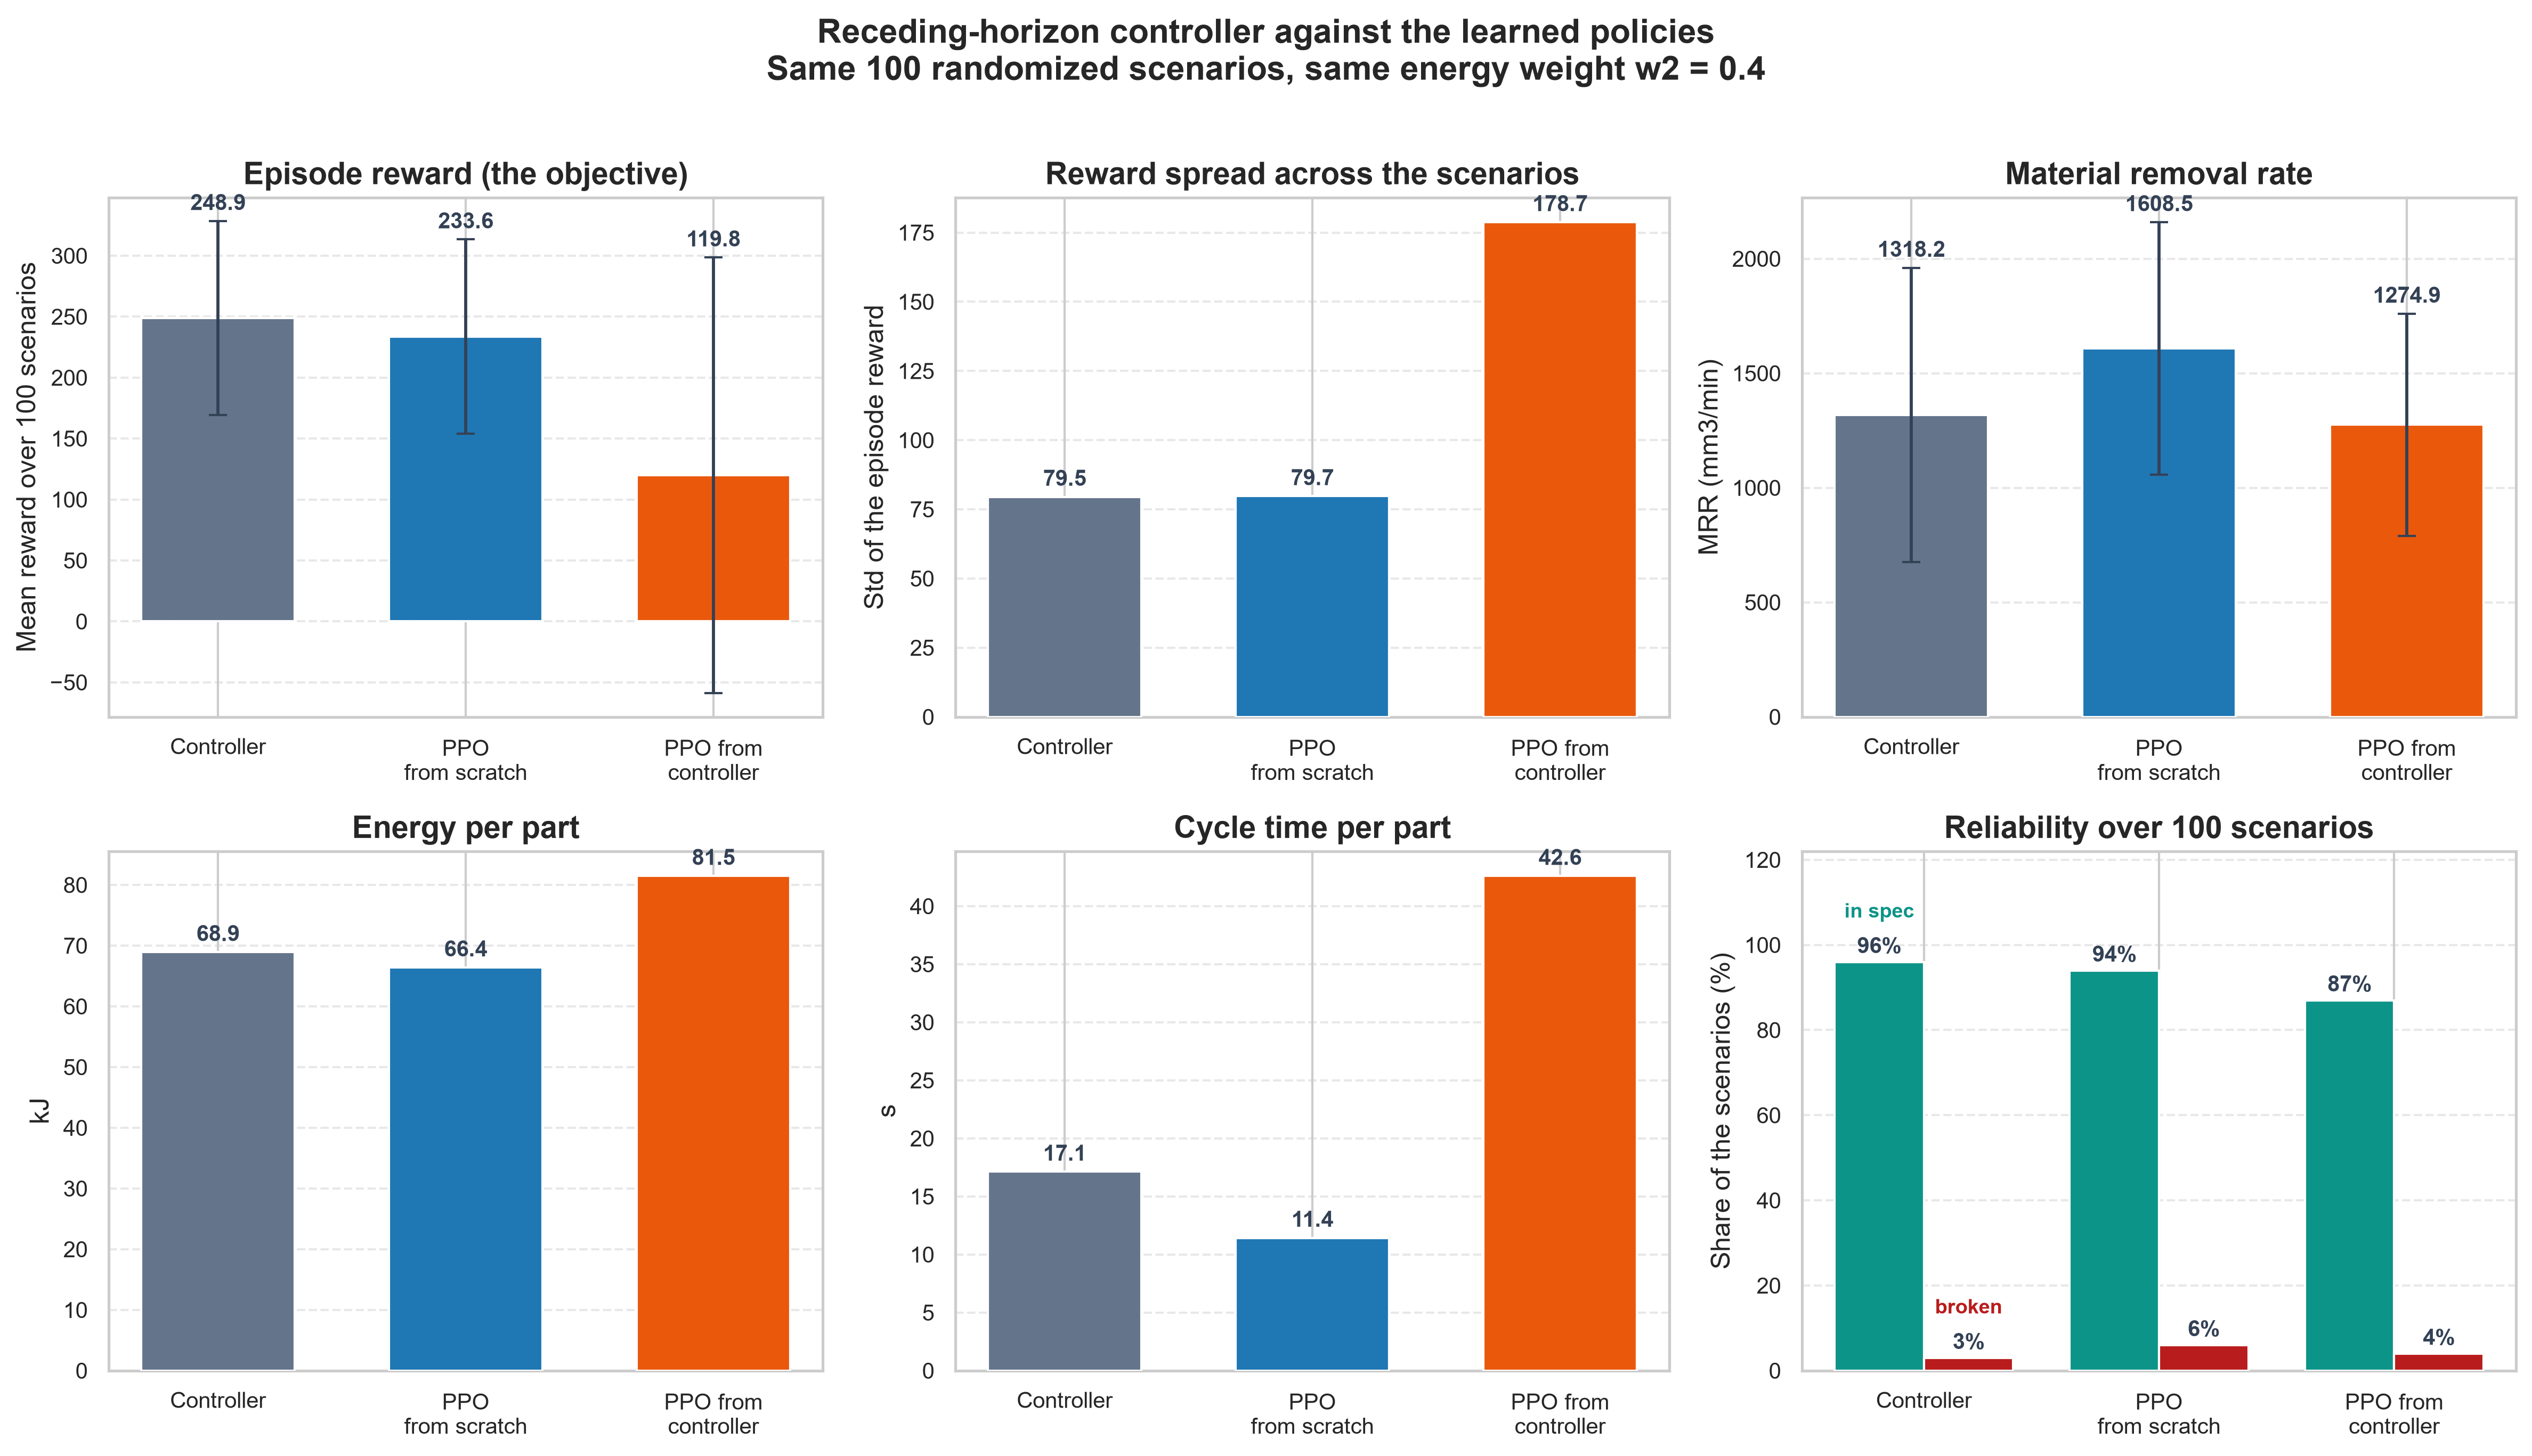
\includegraphics[width=\textwidth,height=0.66\textheight,keepaspectratio]{controller_vs_ppo.png}

    \vspace{0.3em}
    {\footnotesize
    Six panels, too detailed to read at slide size: the values are in the table.
    \alert{The three arms are level on the reward}, and the spread over the 100 scenarios separates them:
    65.9, 30.0, \alert{3.4}. The controller is ahead on the removal rate and the cycle time, the two
    learned policies ahead on the reliability.}
\end{frame}

\begin{frame}{Transfer Experiment: Cross-Material Adaptation}
    \small
    \footnotesize
    \textbf{Target material (harder alloy, same machine):} $k_1 \times 1.25$, $k_2 \times 1.30$,
    $C_\text{wear} \times 2.0$. The source policy was trained for 300,000 steps on the nominal
    material; the adaptation budget on the target is 50,000 steps.

    \vspace{0.4em}
    \centering
    \scriptsize
    \begin{tabular}{@{}lcccc@{}}
    \toprule
    \textbf{Arm} & \textbf{Reward} & \makecell{\textbf{$\Ra$ viol.}\\worst pass} & \makecell{\textbf{$\Ra$ viol.}\\finished surface} & \makecell{\textbf{Parts}\\completed} \\
    \midrule
    Source policy, zero shot & 182.5 & 100.0\% & 3.3\% & 93.3\% \\
    Source policy, fine tuned (50k) & 196.6 & 0.0\% & 0.0\% & 100.0\% \\
    Trained on the target from scratch (50k) & 196.6 & 0.0\% & 0.0\% & 100.0\% \\
    \textbf{Production policy, zero shot} & \textbf{200.3} & 60.0\% & \alert{0.0\%} & 100.0\% \\
    \bottomrule
    \end{tabular}

    \vspace{0.5em}
    \begin{block}{How to read this}
    \footnotesize
    The production policy was trained across a \textbf{distribution of materials} with the material
    context in its observation, so the harder material is inside its training distribution and it
    needs \alert{no adaptation at all}. It scores the highest reward (200.3) and the finished
    surface is in spec in every scenario; its 60\% worst-pass violations fall on the roughing
    passes, which the reward does not constrain: the finished surface, which is the part quality,
    is in spec everywhere. The nominal-trained source policy cannot do this: 182.5, and it violates
    the roughness limit on the worst pass in every scenario. Fine tuning it for 50,000 steps, or
    training on the target from scratch, both fix it, and both land at 196.6.
    \end{block}
\end{frame}

% ========================================================================
% SECTION 7: WORKSTATION
% ========================================================================
\section{Interactive Workstation}

\begin{frame}{Streamlit Digital Twin Workstation}
    \begin{itemize}
        \item \textbf{2D Stock Depletion:} Cylindrical billet cross-section; pass-by-pass cutout; remaining $\kappa$, $a_p$; tool engagement
        \item \textbf{Micro-Topography:} Feed-mark cusp $y_{\text{cusp}}(x) \approx x^2/(8 r_\epsilon) + \text{noise}$; ISO 1302 $\Ra$ overlay; 1.6 $\mu$m ceiling
        \item \textbf{G-Code Generator:} ISO 6983 Fanuc/Siemens compliant; exact PPO sequence; tool/diameter aware
        \item \textbf{Multi-Controller:} Side-by-side PPO vs NSGA-II vs Rule-Based vs Constant-High; live telemetry
        \item \textbf{Cached Loading:} \texttt{@st.cache\_resource} loads model once per session
    \end{itemize}

    \vspace{1em}
    \centering
    \texttt{streamlit run app.py}
\end{frame}

% ========================================================================
% SECTION 8: SOFTWARE ENGINEERING
% ========================================================================
\section{Software Engineering}

\begin{frame}{Architecture \& Reproducibility}
    \footnotesize
    \begin{columns}[T]
        \begin{column}{0.5\textwidth}
            \textbf{Module Structure}
            \begin{itemize}
                \item \texttt{MillingDT/}: config, env, agent (controller init), baselines, sim, utils
                \item \texttt{experiments/}: train, eval, ablation, baselines, transfer, controller, pipeline
                \item \texttt{viz/}: shared plotting utilities
                \item \texttt{results/}: one directory per run (models, log, metrics, plots)
            \end{itemize}

            \textbf{Reproducibility}
            \begin{itemize}
                \item Global seeding (Python, NumPy, PyTorch, CUDA)
                \item Shared scenario tables (train = eval)
                \item \texttt{experiments/summarize\_results.py} regenerates \texttt{RESULTS.md}
            \end{itemize}
        \end{column}
        \begin{column}{0.5\textwidth}
            \textbf{Test Coverage (34 tests)}
            \begin{itemize}
                \item 22 env tests: clipping, truncation, soft norm, 11-D observation, constants, overrides, energy norm, Gym checker, randomization, pinned values, scenario scales, context (weight, material), speed dependence, energy minimum, shared physics
                \item 2 reward tests: golden values ($w_2 = 0.0, 0.4, 0.75$), finishing penalty
                \item 5 integration: train$\to$eval roundtrip, one registration, context in the observation, one policy at a pinned weight, baseline artifact
                \item 3 callback: heartbeat, failure report, interval
                \item 2 training: convergence, reproducibility
            \end{itemize}

            \textbf{Code Quality}
            \begin{itemize}
                \item No unused imports (AST verified)
                \item Constants and paths in \texttt{MillingDT/config/}
            \end{itemize}
        \end{column}
    \end{columns}
\end{frame}

% ========================================================================
% SECTION 9: DISCUSSION
% ========================================================================
\section{Discussion}

\begin{frame}{Discussion}
    \footnotesize
    \begin{columns}[T]
        \begin{column}{0.33\textwidth}
            \begin{block}{What Worked}
            \begin{itemize}
                \item Speed-dependent $k_c$ creates genuine trade-off
                \item Domain randomization $\to$ 99\% completion, 0\% finished violations
                \item One policy beats the 21 per-weight policies
                \item Training across materials makes adaptation unnecessary
                \item Receding-horizon = strong, fair baseline
                \item Controller initialization buys consistency: reward std 30.0 $\to$ 3.4, no breakage            \end{itemize}
            \end{block}
        \end{column}
        \begin{column}{0.33\textwidth}
            \begin{alertblock}{Limitations}
            \begin{itemize}
                \item PPO is level with receding-horizon, not ahead of it
                \item Initializing from the controller does not close the gap: more uniform, but 6.6\% less removal rate and 12.9\% more energy
                \item Ablation: 150k steps/weight (vs 1M production)
                \item Reward charges a pass, metric is a part
                \item Sim-only, no real calibration yet
            \end{itemize}
            \end{alertblock}
        \end{column}
        \begin{column}{0.33\textwidth}
            \begin{exampleblock}{Future Work}
            \begin{itemize}
                \item Compare against a restricted controller (is the gap an information gap?)
                \item Sim-to-real: calibrate, add noise/delay
                \item True multi-objective RL (Pareto, hypervolume)
                \item Online $w_2$ adaptation for energy budget
            \end{itemize}
            \end{exampleblock}
        \end{column}
    \end{columns}
\end{frame}

% ========================================================================
% SECTION 10: CONCLUSION
% ========================================================================
\section{Conclusion}

\begin{frame}{Conclusion}
    \scriptsize
    \begin{itemize}
        \item \textbf{Digital Twin} with speed-dependent cutting energy, tool wear, roughness, stochastic breakage
        \item \textbf{One Gymnasium Environment} (\texttt{MillingDTEnv-v1}) with domain randomization and an 11-D observation that always carries the context
        \item \textbf{One Production Policy} (1M steps): the energy weight is a runtime query, not a retrain
        \item \textbf{Rigorous Evaluation}: Monte Carlo (100 scenarios, 95\% CIs), ablation frontier, weight sweep against the 21 per-weight policies
        \item \textbf{Baselines}: six policies on the same 50 episodes, level on the reward, so no RL advantage yet
        \item \textbf{Controller Initialization}: more uniform (reward std 3.4 against 30.0), no tool breakage, but the controller still removes 38\% more material per minute
        \item \textbf{Transfer Experiment}: the production policy needs no adaptation; the nominal-trained one does
        \item \textbf{Interactive Workstation}: 2D stock depletion, micro-topography, G-code, multi-controller comparison
        \item \textbf{Full Reproducibility}: every result table from committed artifacts by one script
    \end{itemize}

    \vspace{0.2em}
    \begin{alertblock}{Key Scientific Finding}
    \scriptsize
    The speed-dependent specific cutting energy creates a \textbf{genuine energy/throughput trade-off}, and DRL learns to navigate it pass-by-pass while respecting surface quality and tool life constraints. Across the measured frontier the removal rate falls \alert{8.4\%} while the energy of the part falls \alert{9.5\%}. One conditioned policy reaches that whole frontier at runtime, beats the 21 policies trained per weight, and transfers to a harder material with no adaptation.
    \end{alertblock}
\end{frame}

% ========================================================================
% APPENDIX: COMMANDS
% ========================================================================
\appendix
\section{Reproducibility Commands}

\begin{frame}{Key Commands}
    \scriptsize
    \begin{tabular}{@{}ll@{}}
    \toprule
    \textbf{Task} & \textbf{Command} \\
    \midrule
    Tests & \texttt{pytest tests/ -v} \\
    Production & \texttt{python -m experiments.train\_rl --steps 1000000 --seed 42 --randomize --randomize-weight} \\
    Pinned weight & \texttt{python -m experiments.train\_rl --steps 150000 --seed 42 --randomize --w2 0.6} \\
    Ablation grid & \texttt{python -m experiments.train\_rl\_ablation --steps 150000 --scenarios 50 --slots 7} \\
    MC eval & \texttt{python -m experiments.evaluate --scenarios 100} \\
    Weight sweep & \texttt{python -m experiments.evaluate --sweep-weight --scenarios 100} \\
    Compare & \texttt{python -m experiments.evaluate --compare-only} \\
    Baselines & \texttt{python -m experiments.run\_baselines} \\
    Transfer & \texttt{python -m experiments.transfer\_experiment 300000 50000} \\
    Controller init & \texttt{python -m experiments.controller\_experiment 1000000 2000} \\
    Results & \texttt{python -m experiments.summarize\_results} \\
    Workstation & \texttt{streamlit run app.py} \\
    Full pipeline & \texttt{python -m experiments.run\_pipeline --steps 1000000} \\
    \bottomrule
    \end{tabular}
\end{frame}

% ========================================================================
% THANK YOU
% ========================================================================
% THANK YOU
% ========================================================================
\begin{frame}
    \centering
    \vfill
    \Huge \textbf{Thank You}
    \vspace{1em}

    \Large Questions \& Discussion
    \vspace{2em}

    \large Repository: \texttt{G:/My Drive/IITM/AI in Mfg} \\
    ME6324 -- AI in Manufacturing \textbar\ IIT Madras
    \vfill
\end{frame}

\end{document}
